
\hypertarget{menu_project}{}
\section{Project}
\index{project menu}

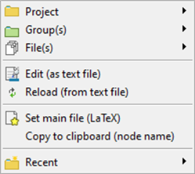
\includegraphics[scale=0.50]{./res/menu_project.png}\\

\begin{scriptsize}\begin{tabularx}{\textwidth}{>{\hsize=0.3\hsize}X>{\hsize=0.8\hsize}X}\\
    \hline
    \textbf{Option} & \textbf{Description} \\
    \hline
    Project & \textit{\href{\#menu\_project\_project}{See options ...}} \\
    Group(s) & \textit{\href{\#menu\_project\_group}{See options ...}} \\
    File(s) & \textit{\href{\#menu\_project\_file}{See options ...}} \\
    \hdashline[1pt/1pt]
    Edit (as text file) & Opens the textual description of the project for editing \\
    Reload (from text file) & Reloads the graphical project interface from the
     textual description of the project \\
    \hdashline[1pt/1pt]
    Set main file (\LaTeX) & Sets (in the current project) the main \LaTeX ~project file \\
    Copy to clipboard (node name) & Copy project node name to Windows clipboard \\
    \hdashline[1pt/1pt]
    Recent & The option will display a Most Recently Used (MRU) project file list.
     Selecting one of the displayed files will open that file \\
    \hline
  \end{tabularx}\end{scriptsize}


\hypertarget{menu_project_project}{}
\subsection{Project}
\index{project menu!project}

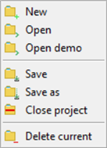
\includegraphics[scale=0.50]{./res/menu_project_project.png}\\

\begin{scriptsize}\begin{tabularx}{\textwidth}{>{\hsize=0.2\hsize}X>{\hsize=0.8\hsize}X}\\
    \hline
    \textbf{Option} & \textbf{Description} \\
    \hline
    New & Creates new project. If you have an open unsaved project you will be prompted to save the project file \\
    Open & Opens existing project and restores the project's state \\
    Open demo & Opens existing demo project and restores the project's state \\
    \hdashline[1pt/1pt]
    Save & Saves the project file \\
    Save as & Saves the current file with a new name \\
    Close project & This option will close any files that are in a virtual folder \\
    \hdashline[1pt/1pt]
    Delete current & This option will delete the virtual folder of the current project \\
    \hline
  \end{tabularx}\end{scriptsize}


\newpage
\hypertarget{menu_project_group}{}
\subsection{Group(s)}
\index{project menu!group}

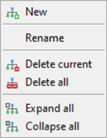
\includegraphics[scale=0.50]{./res/menu_project_group.png}\\

\begin{scriptsize}\begin{tabularx}{\textwidth}{>{\hsize=0.2\hsize}X>{\hsize=0.8\hsize}X}\\
    \hline
    \textbf{Option} & \textbf{Description} \\
    \hline
    New & Creates a new group of current project \\
    \hdashline[1pt/1pt]
    Rename & Renames a selected group of current project \\
    \hdashline[1pt/1pt]
    Delete current & Removes the selected group from the current project \\
    Delete all & Removes all groups from the current project \\
    \hdashline[1pt/1pt]
    Expand all & Expands all groups of the current project in the graphical interface \\
    Collapse all & Collapses all groups of the current project in the graphical interface \\
    \hline
  \end{tabularx}\end{scriptsize}


\hypertarget{menu_project_file}{}
\subsection{File(s)}
\index{project menu!file}

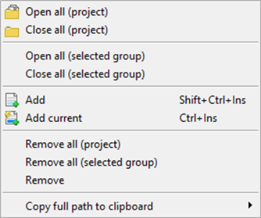
\includegraphics[scale=0.50]{./res/menu_project_file.png}\\

\begin{scriptsize}\begin{tabularx}{\textwidth}{>{\hsize=0.4\hsize}X>{\hsize=0.7\hsize}X}\\
    \hline
    \textbf{Option} & \textbf{Description} \\
    \hline
    Open all (project) & Opens all files of a project \\
    Close all (project) & Closes all files of a project \\
    \hdashline[1pt/1pt]
    Open all (selected group) & Opens all files of a selected group \\
    Close all (selected group) & Closes all files of a selected group \\
    \hdashline[1pt/1pt]
    Add & Opens the windows interface to select file(s) and add the selected(s) files to a selected group \\
    Add current & Add the current file to the selected group \\
    \hdashline[1pt/1pt]
    Remove all (project) & Removes all files from the project \\
    Remove all (selected group) & Removes all files from the selected group \\
    Remove & Removes selected file \\
    \hdashline[1pt/1pt]
    Copy full path to clipboard & \textit{\href{\#menu\_project_file\_copyfullpath}{See options ...}} \\
    \hline
  \end{tabularx}\end{scriptsize}

\hypertarget{menu_project_file_copyfullpath}{}
\subsection{Copy full path to clipboard}
\index{file menu!copy to clipboard}


\includegraphics[scale=0.50]{./res/menu_file_copyfullpathtoclipboard.png}\\

\begin{scriptsize}
  \begin{tabularx}{\textwidth}{>{\hsize=0.3\hsize}X>{\hsize=0.8\hsize}X}\\
    \hline
    \textbf{Option} & \textbf{Description} \\
    \hline
    Unix mode ../.. & Copy full path of current file to clipboard in Unix mode ../.. \\
    Windows mode ..$\backslash$.. & Copy full path of current file to clipboard Windows mode ..$\backslash$.. \\
    \hline
  \end{tabularx}
\end{scriptsize}